In this section, the project planning will be reviewed and updated for the mid-term and final report.
The work-flow diagram, work break-down structure and the Gantt chart will be discussed in the following sections.


\section{Work-flow diagram}
To start with, the tasks to be done on the simulator have been updated and presented in more detail. Also, some tasks have been 
changed in the work flow diagram, making them start earlier or later to better enhance the work flow of the project. 
The tasks in the green and blue box are a more detailed explanation of the finalizing of the simulator design and the performing
of the trade off, respectively. Red boxes are tasks which are explicitly needed in the mid-term report. The updated work flow diagram of the mid term report is given in figure \ref{fig:WFmidterm2}.

\begin{figure}
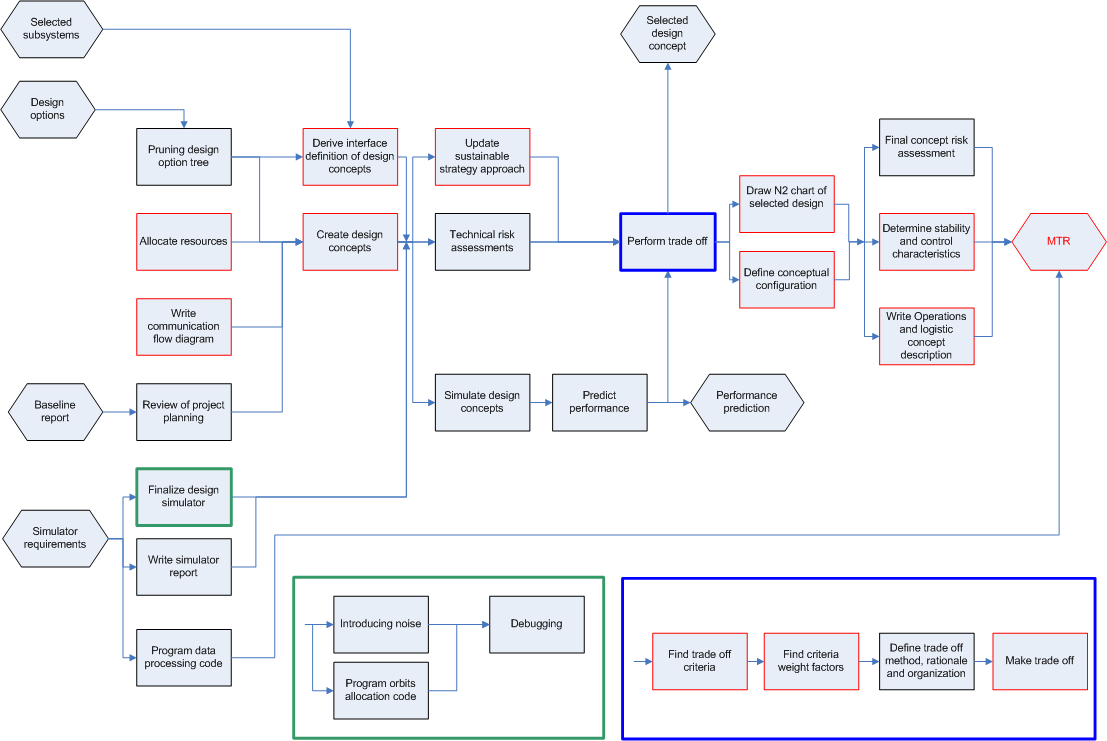
\includegraphics{chapters/img/Workflow_diagram_MTR_v2.jpg}
\caption{Updated work flow diagram for the mid-term report}
\label{fig:WFmidterm2}
\end{figure}

The work-flow diagram of the final report have also been updated. In retrospect, a very important part if the final report was not 
present in the work flow diagram: the finalizing of the design and the feasability determination. Now these tasks have been added
to the daigram to make it complete. As with the work-flow diagram of the mid-term report, all boxes in red are explicitly required
in the final report. The diagram can be seen in figure \ref{fig:WFfinal2}

\begin{figure}
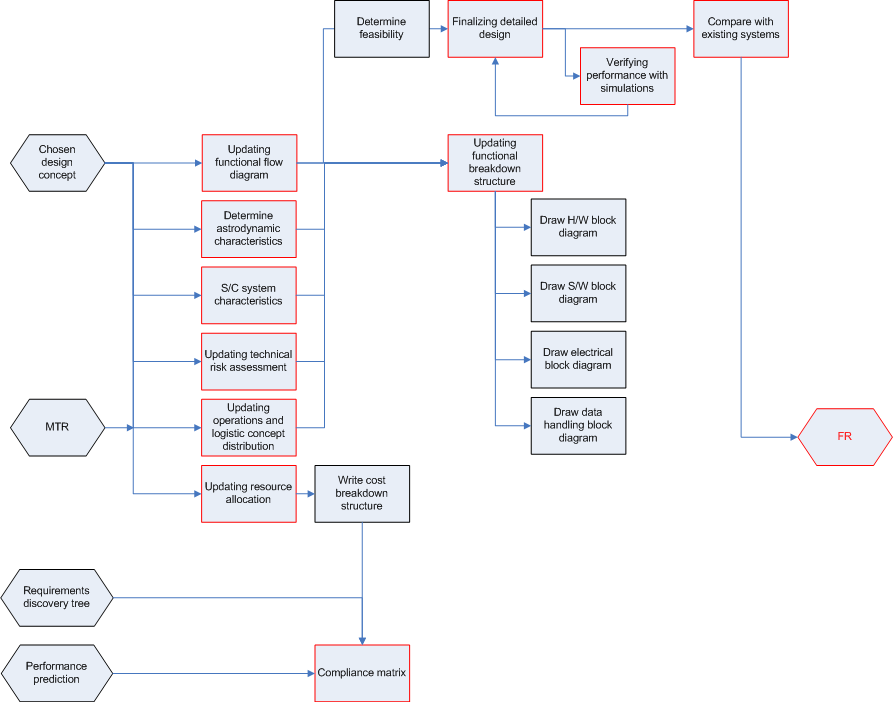
\includegraphics{chapters/img/Workflow_diagram_FR_v2.jpg}
\caption{Updated work flow diagram for the final report}
\label{fig:WFfinal2}
\end{figure}


\ection{Work break-down structure}
The work break-down structures have been updated along with the work flow diagrams. The extra tasks and more detailed tasks
defined in the work-flow diagram have also been added to these structures. Also, the layout has been changed somewhat to make the structure clearer and more correct. The updated work break-down structures can be seen in figures \ref{fig:WBmidterm2} and \ref{fig:WBfinal2}.

\begin{figure}
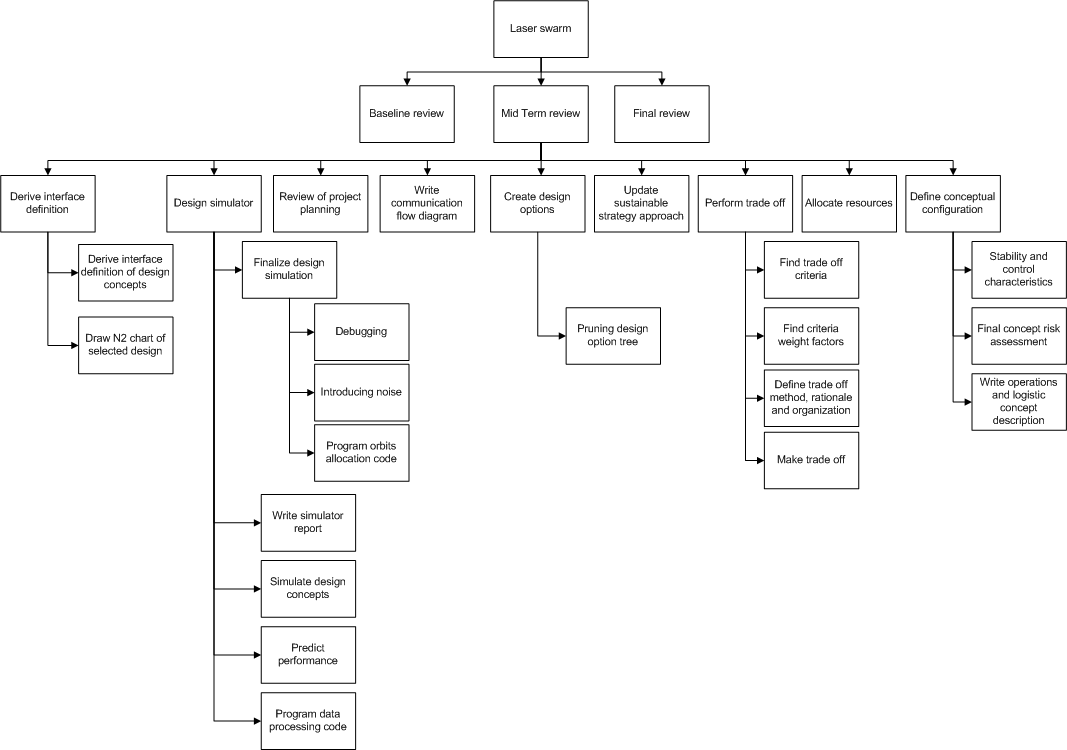
\includegraphics{chapters/img/Workbreakdown_structure_MTR_v2.jpg}
\caption{Updated work break-down structure for the mid-term report}
\label{fig:WBmidterm2}
\end{figure}

\begin{figure}
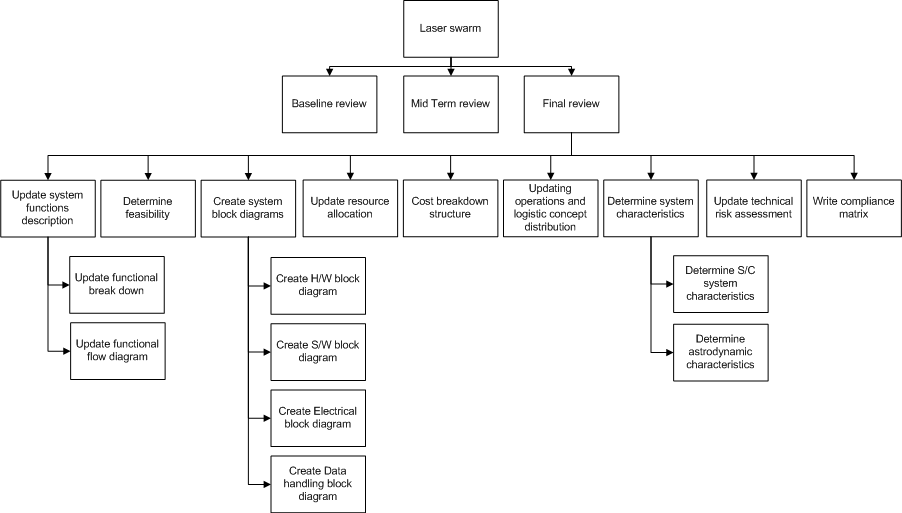
\includegraphics{chapters/img/Workbreakdown_structure_FR_v2.jpg}
\caption{Updated work break-down structure for the final report}
\label{fig:WFfinal2}
\end{figure}

\section{Gantt chart}
As the work flow diagrams and the work break-down structure have been updated, also the Gantt chart has been updated. 
Being further along in the project,it is easier to estimate which tasks needed to be doen for the mid-term and final reports, but also the estimated duration of these tasks was much easier to estimate. The Gantt chart has been updated to contain all the tasks set in the work-flow diagrams. Special care was taken to make sure the Gantt chart was consistent with the work-flow diagrams and the work break-down structures.
This time the simulator tasks were not set apart but integrated with the rest of the project because the simulator is more involved with the 
rest of the project for the mid-term and final reports.
The updated Gantt chart can be seen in figure 

UPDATE THE REFERENCE!!!!!

%\ref{appendixGantt}.